\section{Methoden}

Dieses Kapitel beschreibt nicht das \textsc{Was}, sondern das \textsc{Wie}: Hier soll es nicht um einzelne Features und deren Implementierung gehen, sondern um das Vorgehen beim Planen, Konzipieren, Umsetzen, Testen, Validieren. 

\subsection{Vorgehen}
\label{sec:Vorgehen}

Bei PEAX hat sich die agile Softwareentwicklung nach \textsc{Scrum} durchgesetzt. Da es sich bei \texttt{px} um ein Einzelprojekt handelt, können hier nicht sämtliche Aspekte davon abgebildet werden. Die üblichen \textsc{Scrum}-Rollen wie \textsc{Product Owner} und \textsc{Scrum Master} fallen dabei weg, bzw. bestehen nur in Personalunion des einzigen Entwicklers.

Mit dem Auftraggeber und den Anwendern (Beta-Tester) gibt es aber dennoch Stakeholder, denen der Fortschritt der Arbeit regelmässig berichtet und vorgeführt wird. Von diesen werden auc Rückmeldungen zum Prototyp und zur Projektdokumentation eingefordert, um im weiteren Verlauf des Projekts darauf reagieren zu können.

Die Anwendung soll in mehreren zweiwöchigen Sprints entwickelt werden. Nach jedem Sprint wird der aktuelle Stand an das Entwicklungsteam ausgeliefert. Dabei erhält das Programm einen Versionstag entsprechend der Sprint-Nummer, wozu die Minor-Version erhöht wird (Beispiel: \texttt{v0.1.0} ist der Tag nach dem ersten Sprint, \texttt{v0.3.0} der Stand nach dem dritten Sprint). Bis zum darauffolgenden Sprint ist nun eine Woche Zeit zum Ausprobieren umd zum Erteilen von Rückmeldungen. Diese fliessen in die Planung zum nächsten Sprint ein, der eine Woche nach dem vorausgegangenen Sprint-Ende startet.

Das Backlog wurde zu Beginn des Projekts nur grob skizziert, wird aber vor Beginn eines jeden Sprints dafür detailliert ausgearbeitet. Neben der der Story-Beschreibung nach der Form \textit{Als [Rolle] möchte ich [Funktion], damit [Nutzen]} werden zu jeder Story mehrere Akzeptanzkriterien festgehalten.

Während dem Umsetzen und Testen werden dann zu jeder Story Umsetzungsnotizen und ein Testprotokoll festgehalten. Die Umsetzungsnotizen fliessen jeweils nach dem Sprint in die Dokumentation ein. Ein Story-übergreifender Test-Plan soll nicht erstellt werden. Die Teststrategie wird im folgenden Unterkapitel beschrieben.

Das Projekt entstammt dem PEAX-Ideation-Prozess, und soll auch in diesem Rahmen validiert werden. Dieser Hintergrund ist im ersten Meilensteinbericht (siehe \secref{apx:WeitereDokumente}) genauer beschrieben.

\subsection{Teststrategie}

Wie im Vorsemester im Modul \textit{Software Testing} eingeübt, sollen die \textit{Agile Test Quadrants} (\imgref{fig:agile-testing-quadrants}) als Grundlage zur Erarbeitung einer Teststrategie dienen \cite[S. 242]{agiletest}.

Für die vier Quadranten bieten sich für das vorliegende Projekt verschiedene Arten von Tests an. Diese werden im Folgenden für die einzelnen Quadranten beschrieben.

\begin{figure}
	\centering
	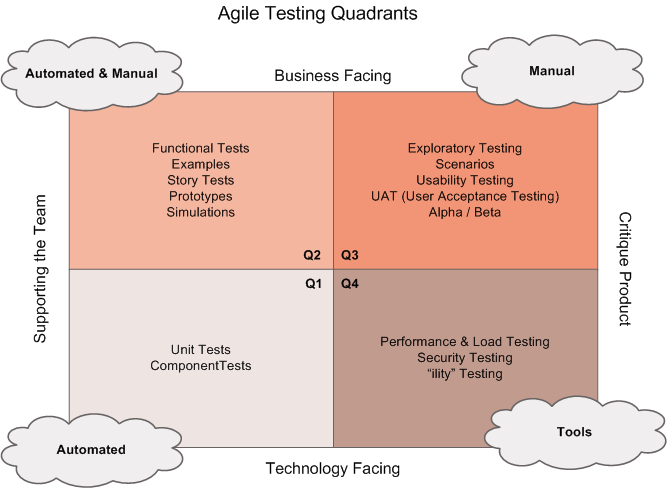
\includegraphics[width=\linewidth]{pics/agile-testing-quadrants.png}
	\caption{\textit{Agile Testing Quadrants} nach Lisa Crispin (\url{https://lisacrispin.com/2011/11/08/using-the-agile-testing-quadrants/})}
	\label{fig:agile-testing-quadrants}
\end{figure}

\subsubsection{Q1: automatisiert}

Im ersten Quadranten geht es um Tests, die vollautomatisch ausgeführt werden können. Diese Tests sollen in einer CI-Umgebung nach jedem Push und vor jedem Merge durchlaufen. Scheitert ein Test, wird der Entwickler notifiziert. Ein Merge-Request soll nicht ausgeführt werden können, wenn Testfälle im Feature-Branch scheitern, sodass die Tests im Master-Branch immer durchlaufen.

Einzelne Funktionen können durch \textit{Unit Tests} abgedeckt werden. Da die Sichtbarkeitsregeln in Go anders geregelt sind als in Java, und ein Unit Test jeweils zum gleichen Modul wie der zu testende Code gehört, können auch interne Funktionen getestet werden, und nicht nur die vom Modul exportierte Schnittstelle \cite[S. 311]{gopl}. Dies erlaubt ein feingranulareres Testing auf Stufe Unit Test.

Die Komponententests sind dann als Tests einzelner Module und somit als Black-Box-Tests zu verstehen, wobei die exportierte (d.h. öffentliche) Schnittstelle angesprochen wird. Auf Mocking soll hierbei verzichtet werden, da das Schreiben \textit{Test Doubles} (Mocks, Spies, Fakes) Kenntnisse der Implementierung und nicht nur der Schnittstelle erfordert. Ändert sich die Implementierung bei gleichbleibendem (und weiterhin erfülltem) Schnittstellenvertrag, sollte auch ein Komponententest weiterhin funktionieren. Dies ist beim Einsatz von Mocks oft nicht gegeben. Eric Elliot bezeichnet Mocking gar als ein \textit{Code Smell}, das die Struktur des Codes verkompliziere, wo doch \textit{Test Driven Development} dabei helfen solle, Code zu vereinfachen \cite[S. 205]{composingsoftware}, 

Ziel der Unit- und Komponententests ist nicht eine möglichst hohe Codeabdeckung, sondern ein optimales Verhältnis von Aufwand und Ertrag: Zeigt es sich, dass für einzelne Tests mit viel Aufwand eine umfassende Umgebung (im weitesten Sinne) aufgebaut werden muss, soll stattdessen geprüft werden, ob der Code nicht besser mittels Tests des zweiten Quadranten getestet werden soll.

\subsubsection{Q2: automatisiert und manuell}
\label{sec:Testing-Q2}

Im zweiten Quadranten geht es um Tests auf der funktionalen Ebene, die teils automatisch, teils manuell ausgeführt werden.

Da \texttt{px} nicht nur interaktiv, sondern auch in Skripten verwendet werden soll, können komplette Workflows ebenfalls vollautomatisiert durchgetestet werden. Ein folgendes Skript könnte etwa folgenden Ablauf beschreiben:

\begin{itemize}
	\item Einloggen auf einen System mit speziellen Test-Zugangsdaten
	\item Hochladen mehrerer Dokumente inklusive Metadaten mit Abspeicherung der dabei generierten Dokument-UUIDs
	\item Tagging der hochgeladenen Dokumente
	\item Herunterladen der zuvor hochgeladenen Dokumente und Vergleich mit dem ursprünglich hochgeladenen Dokument (etwa per SHA-2-Prüfsumme)
	\item Abfragen der zuvor mitgeschickten Metadaten und Tags; Prüfung derselben gegenüber den Ausgangsdaten
\end{itemize}

Ein solcher Test muss zwangsläufig gegen eine laufendes Umgebung durchgeführt werden. (Ähnliche, aber wesentlich einfachere Abläufe werden bereits mit Uptrends durchgeführt, um die Verfügbarkeit der produktiven Umgebung automatisch zu überprüfen.) Hierbei besteht die Gefahr, dass Testfälle aufgrund eines Fehlers in der entsprechenden Umgebung scheitern, und nicht aufgrund der am Code von \texttt{px} vorgenommenen Änderungen. Im schlimmsten Fall müsste ein Merge-Vorgang auf den Master-Branch aufgrund einer nicht funktionierender Umgebung verzögert werden. Eine pragmatische Lösung wäre es, wenn diese Tests gegen die produktive Umgebung ausgeführt würden. Diese Umgebung ist hoch verfügbar, und bei den seltenen Ausfällen derselben könnte auch notfalls mit einem Merge-Vorgang auf den Master-Branch zugewartet werden.\footnote{Der Autor dieser Zeilen ist u.a. auch für die Verfügbarkeit des Produktivsystems zuständig. Ist diese nicht gegeben, werden Entwicklungsarbeiten erfahrungsgemäss unterbrochen, bis das System wieder vollumfänglich verfügbar ist.} Die Zugangsdaten für ein entsprechendes Testkonto können innerhalb der CI-Umgebung als verschlüsselte Variablen und lokal als Umgebungsvariablen abgelegt werden.

Das Schreiben von Skripts ist meistens ein Prozess, dem üblicherweise mehrere manuelle Durchgänge der auszuführenden Arbeitsschritte vorangeht. Skripts werden häufig dann geschrieben, wenn ein manueller Vorgang die Finger stärker beansprucht als den Kopf, und aufgrund der nachgebenden Achtsamkeit die Gefahr für Flüchtigkeitsfehler besteht. So soll es auch im vorliegenden Projekt gehandhabt werden: Wird ein neues Feature eingebaut, d.h. eine neue \textit{User Story} umgesetzt, und sich das Testing desselben als aufwändig herausstellt, soll ein Testskript geschrieben werden, das dann sogleich in die CI-Pipeline eingebaut werden kann. Manuelle Tests sollen so möglichst bald und unkompliziert in automatisierte überführt werden.

\subsubsection{Q3: manuell}

Nach jedem Sprint erhalten die Entwickler bei PEAX Zugang zum aktuellen Stand der Software mit einem Changelog. Sie haben nun eine Woche Zeit, sich mit den neuen Features vertraut zu machen, und auszuprobieren, ob sich die Software wie gewünscht verhält.

Hier geht es weniger um die Korrektheit gemäss Spezifikation (Akzeptanzkriterien in den User Stories), welche bereits durch Tests in Q1 und Q2 gewährleistet werden sollte, sondern um \textit{User Acceptance Tests}. Hiermit wird geprüft, ob das Inkrement die Bedürfnisse der Benutzer erfüllt und ihren Zielen dient. «Another kind of acceptance testing is \textit{user acceptance testing}. Commonly used in Agile environments, user acceptance testing (UAT) checks that the system meets the goals of the users and operates in a manner acceptable to them \cite[S. 85]{testing}.

Auch soll im Rahmen dieser Tests die \textit{Usability} des Inkrements überprüft werden. Stossen mehrere Tester auf die gleichen Probleme? Wurde ein Feature (z.B. ein Subcommand) schlecht benannt, sodass dessen Semantik unklar ist? Ist die angebotene Hilfe-Funktion zu einem Befehl unklar oder schlecht formuliert?

Die Tests in Q3 sind jeweils in der ersten Wochenhälfte nach einem Sprint durchzuführen, sodass die Rückmeldungen für die Planung des nächsten Sprints, der in der darauffolgenden Woche startet, berücksichtigt werden kann.

\subsubsection{Q4: Tools}

Für die Qualitätssicherung können verschiedene Werkzeuge zum Einsatz kommen:

\begin{description}
	\item[Benchmarks] Bieten sich bei der Implementierung einer performancekritischen Funktion mehrere Varianten an, ist die bessere Variante mithilfe von Benchmarks zu bestimmen. Die integrierte Benchmark-Funktion des \texttt{go}-Tools\footnote{\texttt{go test -bench=[pattern]}}, die eine Funktion so oft laufen lässt, bis eine statistisch relevante Aussage über deren Performance gemacht werden kann, ist hierzu völlig ausreichend \cite[S. 321]{gopl}.
	\item[Profiling] Im Profiling geht es darum, die kritischen Stellen im Code im Bezug auf Rechenzeit, Speicherverbrauch und blockierende Operationen zu ermitteln, um Aufgrund dieser Erkenntnis effektive Optimierungen am Code vornehmen zu können (Flaschenhalsoptimierung). Hierzu bietet das \texttt{go}-Tool\footnote{\texttt{go test -cpuprofile/-memprofile/-blockprofile=[Ausgabedatei]}} wiederum sehr mächtige Werkzeuge out-of-the-box an \cite[S. 324]{gopl}.
	\item[Quellcodeanalyse] Kompilierbarer und korrekter Quellcode ist nicht automatisch auch guter Quellcode im Bezug auf Klarheit, Einfachheit, Eleganz und Best Practices. Beispielsweise sollen nach Möglichkeit keine veralteten und unsicheren APIs verwendet werden. Exportierte Funktionen, d.h. die öffentliche Schnittstelle eines Moduls, muss dokumentiert sein. Hierzu gibt es einerseits das Tool \texttt{go vet}\footnote{Vet examines Go source code and reports suspicious constructs, such as Printf calls whose arguments do not align with the format string.}, das zum Lieferumfang von Go gehört, und potenzielle Fehler im Code meldet. Das Zusatztool \texttt{golint}\footnote{\url{https://github.com/golang/lint}} meldet stilistische Unschönheiten im Code.
\end{description}

Da es bei diesen Tools nicht um kategorische Qualitätskriterien (richtig oder falsch), sondern eher um kontinuierliche (schnell/langsam, hoher/tiefer Speicherverbrauch, hohe/tiefer Quellcodequalität) handelt, die einer subjektiven Interpretation bedürfen, sollen diese Tools nicht Teil der CI-Pipeline sein, sondern kontinuierlich (\texttt{go vet} und \texttt{golint}) und bei konkretem Bedarf (Benchmarking, Profiling) im Entwicklungsprozess eingesetzt werden. Um eine gewisse Quellcodeanalyse gewährleisten zu können, ist die Ausgabe von \texttt{go vet} und \texttt{golint} am Ende eines jeden Sprints summarisch zu dokumentieren.\footnote{Da die Ausformulierung von Rechtfertigungen oftmals anstrengender ist als die notwendigen Korrekturen am Code vorzunehmen, ist diese Massnahme als Anreiz zu verstehen, die erhaltenen Warnungen zu behandeln statt zu ignorieren.}
